\documentclass{article}
\usepackage[utf8]{inputenc}
\usepackage{parskip}
\usepackage{float}
\usepackage{graphicx}
\usepackage{subcaption}
\usepackage{cmbright}
\usepackage{geometry}
 \geometry{
 a4paper,
 total={170mm,257mm},
 left=20mm,
 top=20mm,
 }
 \usepackage{titling}
 \usepackage{hyperref}
 \usepackage{xcolor}
 \usepackage{booktabs}

\usepackage{tikz}
\usetikzlibrary{shapes.geometric, arrows.meta, positioning}

% Red marker for things we still have to do.
% Remove all \todo{...} before submitting.
\newcommand{\todo}[1]{\textcolor{red}{[TODO: #1]}}

\title{Explainable Predictive Process Monitoring}  % REFINE TITLE (e.g., name the XAI technique)
\author{Jerrik Faber, Max Hoijng, Job Oosterkamp, Bora Şenel, Floris Vermeulen}
\date{October 2026}

\usepackage{fancyhdr}
\setlength{\headheight}{14pt}
\fancypagestyle{plain}{%
    \fancyhf{}
    \fancyfoot[R]{\IfFileExists{jads.png}{
\includegraphics[width=2cm]{jads.png}}{}}
    \fancyfoot[L]{\thedate}
    \fancyhead[L]{Process Mining (JM0211)}
    \fancyhead[R]{Group 11}
}
\makeatletter
\def\@maketitle{%
  \newpage
  \null
  \vskip 1em%
  \begin{center}%
  \let \footnote \thanks
    {\LARGE \@title \par}%
    \vskip 1em%
  \end{center}%
  \par
  \vskip 1em}
\makeatother

\begin{document}

\maketitle

\noindent\begin{tabular}{@{}ll}
    Students & \theauthor\\
    Group: & 11\\
    \end{tabular}

% The table of contents is left out on purpose: the short paper has a limit of
% 5 pages excluding references.
% \tableofcontents

% ASSIGNMENT GROUP 11: Explainable Predictive Process Monitoring
% Reproduce a post hoc XAI technique that finds the process features with the
% greatest impact on the predictions of a predictive process monitoring model.
% Contact person: Laura Genga.
% Dates: draft for peer review 28 Oct 23:59, peer feedback 3 Nov 23:59,
% final deliverables 9 Nov 23:59, poster session 12 Nov 13:45.
% Limit: 5 pages excluding references.

% ============================================================
\section{Motivation and Scientific Background}
% ============================================================

Process mining uses the event logs of information systems to analyse and improve processes~\cite{aalst2016}. Predictive process monitoring (PPM) goes one step further and uses historical event data to predict the future of cases that are still running, for example their outcome, so that process owners can intervene before a case ends~\cite{teinemaa2019}. Benchmarks show that black-box models such as XGBoost and random forests predict outcomes accurately~\cite{teinemaa2019}, but they do not show why a case gets a certain prediction. Without that insight an analyst cannot judge whether a prediction can be trusted or what to change in the process. Explainable AI (XAI) addresses this problem~\cite{arrieta2020}, and post hoc methods do so for models that are already trained. Existing post hoc methods show which activities influence a prediction, but not whether it matters \emph{where} in the trace an activity is executed. Vazifehdoostirani et al.~\cite{vazifehdoostirani2024} close this gap with the location permutation importance. We reproduce their technique and change the way the activities to test are chosen (Section~\ref{sec:approach}).

\paragraph{Use case.}
\todo{Give one concrete example where it matters why a model makes a prediction.}

\paragraph{Embedding in the course.}
\todo{Say where predictive process monitoring fits in the course and where our XAI technique fits in.}

\paragraph{Commonalities and differences.}
\todo{Compare our topic to the other groups. Groups 9 and 10 also do predictive process monitoring (trace clustering with LLMs, inter-case features) and Group 7 does prescriptive monitoring. What is the same and what is different?}

% ============================================================
\section{Conceptual Approach}
\label{sec:approach}
% ============================================================

We reproduce the post hoc XAI technique of Vazifehdoostirani et al.~\cite{vazifehdoostirani2024}. It measures how much the \emph{location} of activities in a trace matters for an outcome prediction model, in the spirit of permutation feature importance: if we shuffle the locations of a group of activities (an itemset) and the model gets worse, the location of that itemset matters. We change one step, the choice of the itemsets, and compare the results (Figure~\ref{fig:approach}).

\paragraph{Input.}
An event log with, for every case, the activities in execution order and a binary outcome label. Timestamps only order the events, and resources are not used. The variant of step 2 also needs case attributes for its case-distance measure (for BPIC11: age, diagnosis, diagnosis code, specialism code, treatment code). Traces are encoded with index-based encoding: position $i$ of the trace is a feature that holds the activity at that position. The method does not depend on the model type, and like the original paper we use XGBoost.

\paragraph{Parameters.}
Table~\ref{tab:parameters} lists the parameters and the values we use.

\begin{table}[H]
    \centering
    \caption{Parameters of the approach.}
    \label{tab:parameters}
    \small
    \begin{tabular}{@{}p{3.3cm}p{8.3cm}p{3.2cm}@{}}
        \toprule
        Parameter & Meaning & Value \\
        \midrule
        Itemset strategy & How the itemsets are chosen & A: Apriori, B: IMPresseD \\
        Minimum support, top $k$ (A) & Smallest share of cases that contain an itemset, and number of itemsets with more than one activity that are kept & 0.5 and 10 (also 0.2 and 25) \\
        Pattern length (B) & Longest pattern; every extension step adds one activity & 3 \\
        Extension rules (B) & A pattern is extended by an activity that directly or eventually follows or precedes it & all four \\
        Feasibility, order preservation & Keep the permuted traces realistic (step 3) & on \\
        Folds, repetitions & Cross-validation folds, and random permutations per itemset & 5 and 10 \\
        Test size, seed & Share of cases held out for the itemset selection, and the random seed & 0.2 and 42 \\
        \bottomrule
    \end{tabular}
\end{table}

\paragraph{Steps and methods.}
\begin{enumerate}
    \item \textbf{Baseline.} Train the model on the index-encoded log and measure its F1-score with cross-validation.
    \item \textbf{Itemset selection.} Choose the activity sets whose location will be tested. The original method uses Apriori. Our variant uses the outcome-oriented patterns of IMPresseD~\cite{vazifehdoostirani2023}. Both give a list of activity sets, and the rest of the pipeline stays the same.
    \item \textbf{Location permutation.} For each itemset, shuffle the locations of its activities over the traces. A new location of an activity must be a location where that activity occurs somewhere in the log (feasibility), and the order of the activities within the itemset stays the same (order preservation). Then encode the permuted log again.
    \item \textbf{Importance.} Score the permuted log with the model from step 1. The drop in F1 compared with the baseline is the importance of the location of the itemset. The shuffle is random, so it is repeated 10 times.
\end{enumerate}

\emph{Strategy A: Apriori.} Every single activity is analysed, together with the most frequent itemsets of two or three activities. Apriori searches level by level for sets that occur in at least the minimum support of the cases, using the rule that every subset of a frequent set must be frequent too.

\emph{Strategy B: IMPresseD.} A pattern is a chain of activities in which neighbours are related directly (the second follows immediately) or eventually (it follows later, with at least one event in between). Every pattern is scored on three interest functions: \emph{case coverage} (share of cases that contain it, to maximise), \emph{outcome interest} (information gain of the outcome label from the number of times the pattern occurs in a case, to maximise) and \emph{case distance} (mean distance between cases with and without the pattern based on case attributes, to minimise; this lowers the risk that a pattern only looks important because of, for example, the age of the patients). A pattern is dropped if another pattern is at least as good on all three functions and strictly better on one. The patterns that remain form the Pareto front, so no threshold has to be chosen. Starting from all single activities, the patterns of the front are extended by one activity and scored again, up to length 3. The assignment asks for activity sets, so the ordering relations are dropped at the end: A$\to$B, B$\to$A and A$\Rightarrow$B all give $\{A,B\}$, and duplicates are removed. The patterns are discovered on the training part of the log only, because the outcome interest uses the labels and the choice of itemsets should carry no information about the test cases.

\paragraph{Output.}
For every itemset, a distribution of F1 drops: how much the location of that itemset matters for the predictions. We get this for the itemsets of both strategies, which lets us check whether the same activities and locations come out as important, and how many itemsets each strategy needs.

\begin{figure}[H]
    \centering
    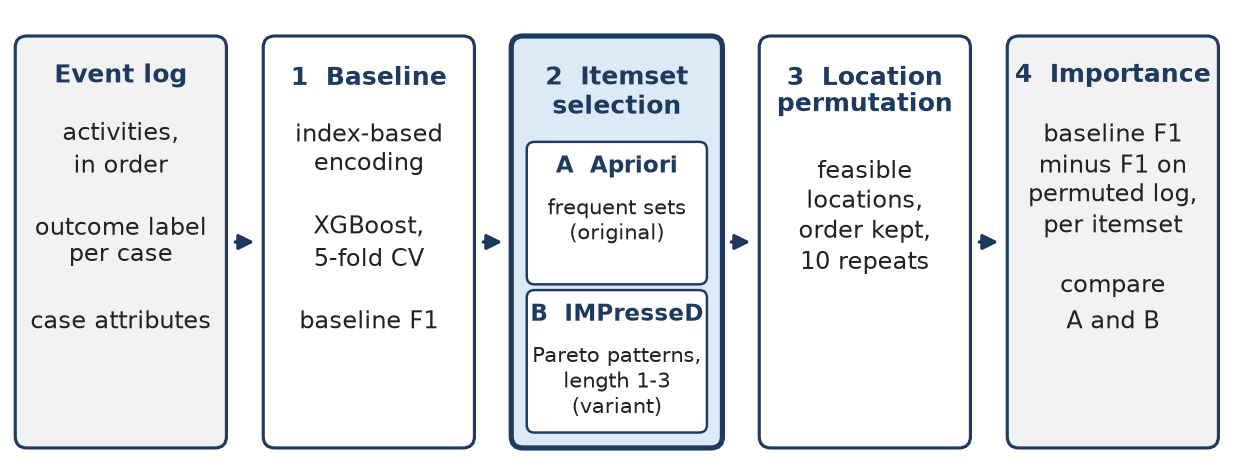
\includegraphics[width=\textwidth]{figures/figure1_approach.png}
    \caption{The approach. Strategy A (Apriori) and strategy B (IMPresseD) both give a list of itemsets for step 2. The other steps are the same for both.}
    \label{fig:approach}
\end{figure}

% ============================================================
\section{Implementation}
% ============================================================

\label{sec:implementation}

The approach is implemented in Python~3. Structure and function names follow the code of the original authors~\cite{vazifehdoostirani2024,vazifehdoostirani2023}\footnote{\url{https://github.com/MozhganVD/PermutationLocationImportance} and \url{https://github.com/MozhganVD/InteractivePatternDetection}}, so that every reproduced step can be compared with the original; our additions are kept in a separate folder. One command, \texttt{python main.py}, runs all steps for all event logs, with the parameters read from a YAML configuration file. Table~\ref{tab:implementation} links the steps of Section~\ref{sec:approach} to the code.

\begin{table}[H]
    \centering
    \caption{Implementation of the steps of the approach.}
    \label{tab:implementation}
    \small
    \begin{tabular}{@{}p{3.6cm}p{6.6cm}p{4.4cm}@{}}
        \toprule
        Step & Module (main functions) & Libraries \\
        \midrule
        Loading and preprocessing & \texttt{tools.py} (\texttt{DataManager}) & pm4py, pandas \\
        1. Baseline model & \texttt{cross\_validation\_process\_permutation.py}, \texttt{tools.py} (\texttt{index\_encoding}) & XGBoost, scikit-learn \\
        2A. Apriori & \texttt{tools.py} (\texttt{frequent\_activity\_sets}) & mlxtend \\
        2B. IMPresseD & \texttt{auto\_impid.py}, \texttt{imipd.py} & networkx, paretoset, scikit-learn, SciPy \\
        3--4. Permutation, importance & \texttt{tools.py} (\texttt{shuffle\_sequence}, \texttt{trace/itemset\_permutation\_importance}) & NumPy, scikit-learn \\
        \bottomrule
    \end{tabular}
\end{table}

\paragraph{Event log and model.}
The logs are loaded and filtered with pm4py~\cite{berti2019}. As in the original code, activity names are normalised and cases with an activity that occurs fewer than twice in the log are removed. The BPIC11 timestamps only record the date (87--89\% of consecutive events in a case share one), so the events are ordered by their event number. The index-based encoding is implemented as one binary feature per pair of position and activity. The model is XGBoost~\cite{chen2016} with default parameters, evaluated with stratified 5-fold cross-validation and the weighted F1-score (scikit-learn~\cite{pedregosa2011}).

\paragraph{Itemset selection.}
Strategy A applies the Apriori implementation of mlxtend to all cases. Strategy B ports the automatic mode of the IMPresseD tool: every trace is a chain graph, outcome interest is computed as mutual information, the distance between two cases is $(m \cdot \text{Jaccard} + \text{Euclidean}_{[0,1]})/(m+1)$ over $m$ categorical attributes and the min-max scaled numeric ones, and the Pareto front is computed with paretoset. As in the tool, patterns with an eventual relation are not extended further. We deviate from the tool in two places: the rule that adds a predecessor and a successor in one step is switched off, so that every step adds exactly one activity, and the case distance uses only the case attributes, as defined in the paper.

\paragraph{Location permutation and importance.}
An activity is moved to a random location at which it was observed; the activities of an itemset are moved one at a time, each to a location after the previous one, so that their order is kept. Every itemset and repetition starts from the original traces, and the F1 drop is measured on the held-out cases of each fold, with the test F1 of the fold as baseline. A single activity that is moved in fewer than three cases gets importance 0. Itemsets that contain an activity with a fixed location, i.e.\ always at the same position counted from the start or from the end of the trace (such as a start or end activity), are not permuted: their location cannot matter, and moving them would create unrealistic traces. These activities are detected from the log, not named by hand.

\paragraph{Reproducibility.}
All random steps are seeded, including the fold split. We first ported the authors' code literally and verified the port on the same data: it gives the same Apriori itemsets, the same permutations (355 of 355 for itemsets, 218 of 218 for single activities) and the same IMPresseD Pareto patterns. We then corrected three places where the original code deviates from the published method: it measured the F1 drop on the training cases, which the model has largely memorised; it never reset the permuted traces, so the importance of an itemset depended on the itemsets permuted before it; and a bookkeeping error in its shuffle moved a wrong event in 25 of the 355 BPIC11 permutations, breaking the order of the itemset in 9 of them. 30 unit tests cover the components.

% ============================================================
\section{Evaluation Design and Results}
% ============================================================

% Outline: drafts/results_outline.md. Rubric S4 (10 points). Budget: about 1.3 to 1.5 pages,
% two tables and one figure. All numbers must come from a fresh run of main.py on main.

\paragraph{Data.}
\todo{BPIC11 f1, f2, f3: hospital log from the authors' repository, labelled as in Teinemaa et al. One line per log: cases (1130/1130/1111), activities, maximum trace length (36/40/31), share of positive labels (results/summary.csv). Case attributes: refer back to Section 2.}
\todo{Synthetic log and two negative controls (15 cases, 100 events): activity B occurs in every case and only its location decides the label (early 0, late 1, 10\% label noise). Controls: shuffled within case (location removed) and shuffled outcomes (labels permuted). Purpose: test the importance step.}
\todo{Simulated logs: 1000 cases, 10 logs per scenario (pair in 30\% or 60\% of the cases). Planted: x (location), \{p, q\} (location of a pair), y (existence). Purpose: test the selection step.}

\paragraph{Evaluation design.}
\todo{Evaluation questions. E1: does a location effect give a clear F1 drop, and the controls a drop of about 0? E2: does each strategy select the planted itemsets? E3: on BPIC11, does IMPresseD instead of Apriori change which activities and itemsets have an important location, and how many itemsets are needed? E4: does the Apriori baseline change with support 0.2 and top 25?}
\todo{Metrics: weighted test F1 of the model (and train F1); F1 drop per itemset over 50 values (5 folds $\times$ 10 repetitions), mean $\pm$ std and box plots; location recall, existence recall and noise share against the gold standard; number and sizes of itemsets, Jaccard overlap, top-10 overlap and Spearman correlation between strategies.}
\todo{Gold standard: in the synthetic and simulated logs we generate the labels, so the relevant itemsets are known; the controls are a gold standard of ``nothing matters''. BPIC11 has no ground truth, so there the evaluation is a comparison of the strategies, not an accuracy test.}
\todo{Parameters: refer to Table~\ref{tab:parameters}; one sentence of motivation each (authors' defaults for Apriori, length 3 for both strategies, 5 folds and 10 repetitions as in the paper, IMPresseD selection on 80\% because it uses the labels).}

\paragraph{Results.}
\todo{E1: test F1 synthetic 0.65 against 0.39/0.42 for the controls; F1 drop of B against the largest absolute drop in the controls (NEEDS RERUN). Table B.}
\todo{E2: y selected by all strategies in every log; x by all, except IMPresseD in the rare-pair scenario (8 of 10). Failure case: no strategy ever selects \{p, q\}, because Apriori selects on frequency and IMPresseD on presence, while only the location of the pair matters (link to Section 5). Noise share 0.50 IMPresseD against 0.73 Apriori. Table B.}
\todo{E3 selection: IMPresseD selects mostly itemsets of size 2 and 3, Apriori mostly single activities; the multi-activity itemsets hardly overlap (Jaccard 0.00 to 0.02). Model: train F1 0.99 against test 0.90 to 0.93, the reason why the importance is measured on the test folds. Table A.}
\todo{E3 importance (NEEDS RERUN and the comparison code from job/location-importance-comparison): top itemset per strategy and log, top-10 overlap, Spearman on the shared itemsets, IMPresseD itemsets above the best Apriori itemset, number of itemsets and runtime. Figure C: box plots of the top 10 itemsets of both strategies for one log. Interpret one top itemset as in the original paper, and check whether it relates to the activity that defines the label.}
\todo{E4: effect of support 0.2 and top 25 on the number of itemsets and the top itemsets (or only on the selection, if the full run is not feasible).}
\todo{Table A: per BPIC11 log and strategy: itemsets (sizes 1/2/3), Jaccard with Apriori, train/test F1, top itemset and its mean F1 drop, top-10 overlap, Spearman.}
\todo{Table B: synthetic against controls (test F1, F1 drop of B, largest absolute drop in the controls) and simulated recall (location, existence, noise share per strategy).}
\todo{Figure C: box plots from \texttt{results/LOG/STRATEGY\_location\_importance.csv}.}

% ============================================================
\section{Limitations and Future Work}
% ============================================================

\paragraph{Limitations.}
\todo{Limitations of the approach and of the evaluation.}

\paragraph{Future work.}
\todo{Improvement directions.}

% ============================================================
\section*{Technology Statement}
% ============================================================
% Mandatory. Without it the assignment gets 0 points.
% Text from the course syllabus. Fill in the capitalized parts.

During the preparation of this work, I/We used [NAME TOOL / SERVICE / VERSION OF AI TOOL] in order to [REASON]. The following parts of the assignment were affected/generated by AI tool usage: [INTRODUCTION / METHODS / xxx, DISCUSSION]. After using this tool/service, [NAME STUDENT(S)] evaluated the validity of the tool's outputs, including the sources that generative AI tools have used, and edited the content as needed. As a consequence, [NAME STUDENT(S)] take(s) full responsibility for the content of their work.

\bibliographystyle{plain}
\bibliography{references}

\end{document}
